% Author: Dominik Harmim <xharmi00@stud.fit.vutbr.cz>


\documentclass[a4paper, 11pt, twocolumn]{article}


\usepackage[czech]{babel}
\usepackage[utf8]{inputenc}
\usepackage[left=2cm, top=2cm, bottom=3cm, text={17cm, 24cm}]{geometry}
\usepackage{times}
\usepackage{graphicx}


\begin{document}


	\twocolumn[
		\begin{@twocolumnfalse}
			\begin{center}
				{\Large
					Vysoké učení technické v~Brně \\
					Fakulta informačních technologií \\
				}
				{
\includegraphics[width=0.4\linewidth]{inc/FIT_logo.pdf}} \\

				{\LARGE
					Signály a~systémy \\
					Projekt \\[0.4cm]
				}

				{\large
					Dominik Harmim (xharmi00) \\
					\texttt{xharmi00@stud.fit.vutbr.cz} \\
					\today
				}
			\end{center}
		\end{@twocolumnfalse}
	]


	\section*{Řešení}

	Řešeno v~programu \texttt{MATLAB}. Všechny uvedené funkce jsou funkcemi v~tomto programu,
	pokud není řečeno jinak. Obrázky jsou na první pohled možná špatně čitelné, ale jsou ve
	vektorovém formátu, takže je možné hezky si je zvětšit, doufám že s~tím nebude problém.

	Veškeré výpočty jsou v~odevzdaném souboru \texttt{xharmi00.m}.

	\begin{enumerate}
		\item
			Vzorkovací frekvence signálu je \textbf{16\,000~[Hz]}.
			Délka signálu ve vzorcích je \textbf{16\,000}, v~sekunddách \textbf{1~[s]}.
			Zvuk jsem zpracoval funkcí \texttt{audioread}.

		\item
			Spektrum signálu pomocí diskrétní Fourierovy transformace
			jsem spočítal funkcí \texttt{fft}.
			\\ 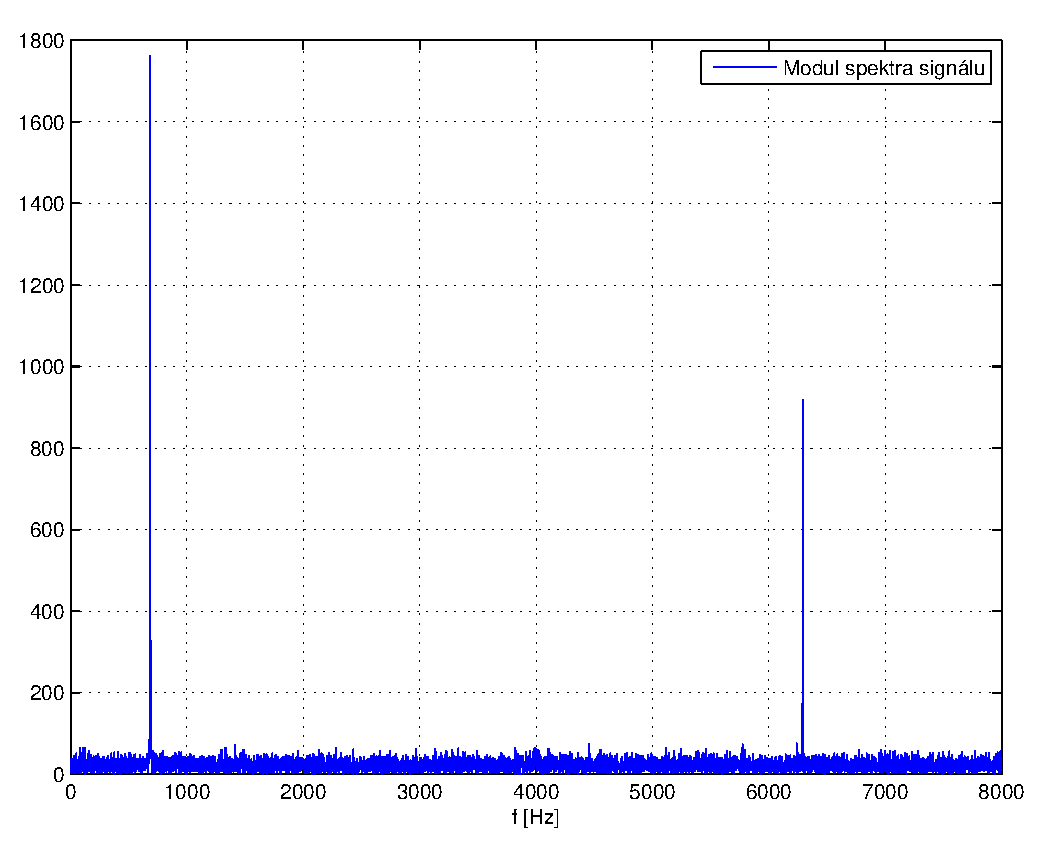
\includegraphics[width=\linewidth]{inc/2.eps}

		\item
			Maximum modulu spektra signálu je na frekvenci \textbf{685~[Hz]}.
			Maximum a~jeho pozici, podle které jsem našel jeho frekvenci jsem našel funkcí \texttt{max}.

		\item
			\textbf{Filtr je stabilní}, protože všechny póly~$ p_k $ jsou uvnitř jednotkové kružnice,
			platí vzath~$ |p_k| < 1 $.
			Obrázek s~nulami a~póly jsem vytvořil funkcí \texttt{zplane}.
			\\ 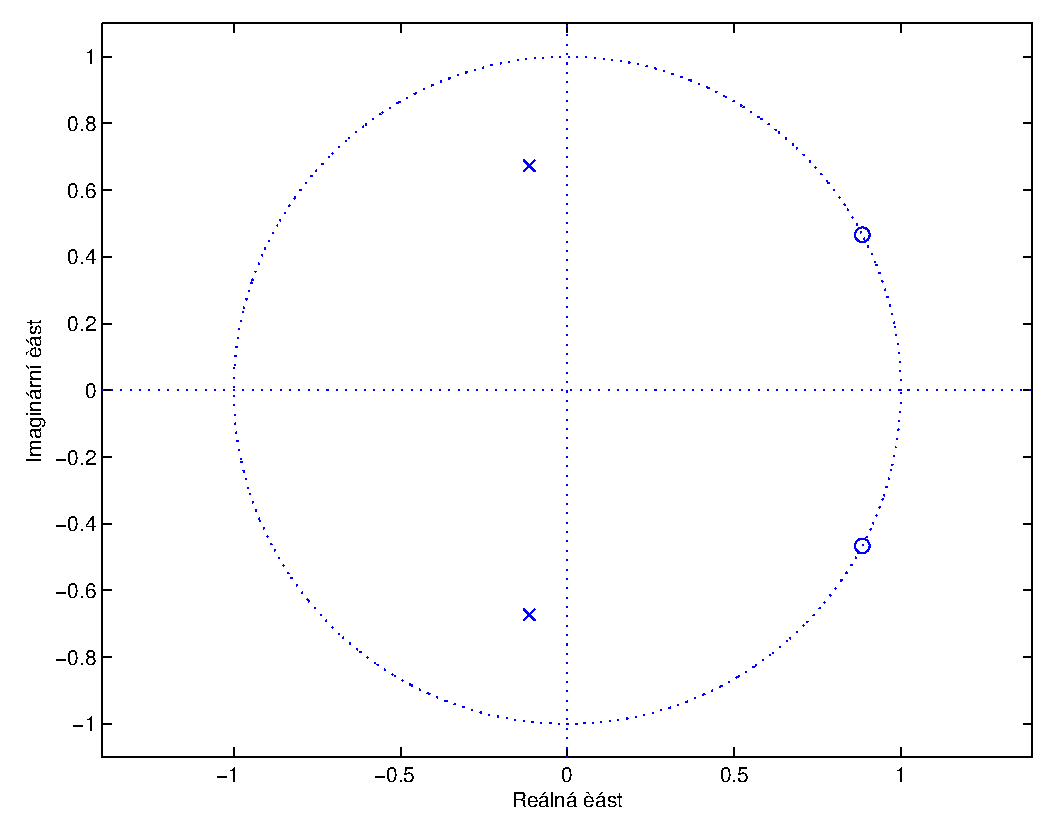
\includegraphics[width=\linewidth]{inc/4.eps}

		\item
			Filtr je typu \textbf{horní propusť}, viz přednáška o~systémech s~diskrétním časem.
			Modul kmitočtové charakteristiky jsem spočítal funkcí \texttt{freqz} s~počtem bodů pro
			zobrazení 256.
			\\ 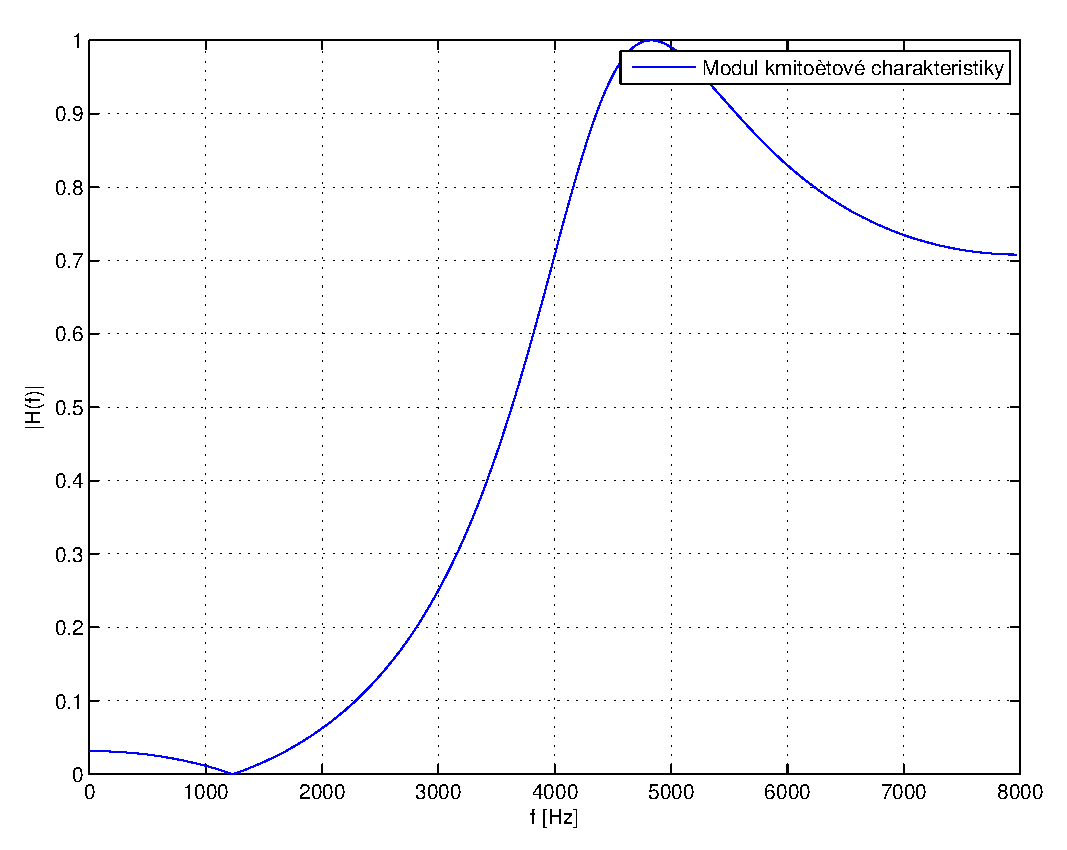
\includegraphics[width=\linewidth]{inc/5.eps}

		\item
			Filtraci jsem provedl funkcí \texttt{filter}. Spektrum signálu pomocí diskrétní
			Fourierovy transformace jsem spočítal funkcí \texttt{fft}.
			\\ 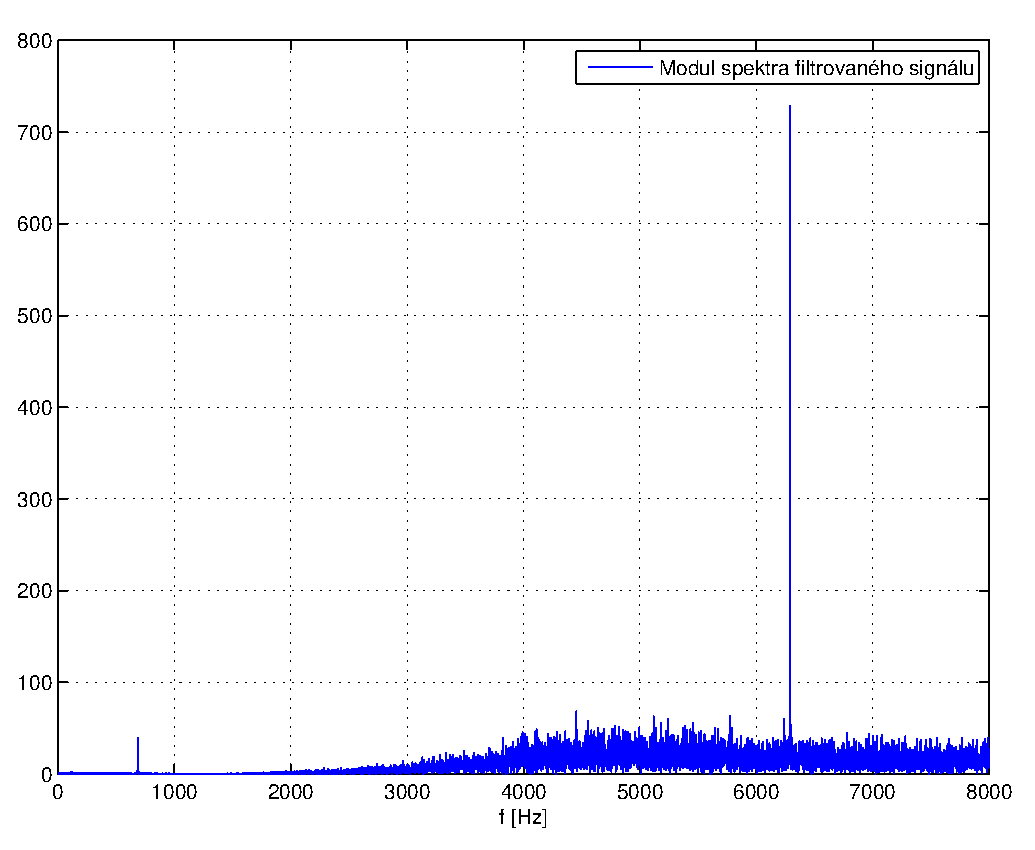
\includegraphics[width=\linewidth]{inc/6.eps}

		\item
			Maximum modulu spektra filtrovaného signálu je na frekvenci \textbf{6\,292~[Hz]}.
			Maximum a~jeho pozici, podle které jsem našel jeho frekvenci jsem našel funkcí \texttt{max}.

		\item
			Obdelníkové implusy se nacházejí na vzorku \textbf{12\,538}, což je čas
			\textbf{0.783625~[s]}, viz obrázek.
			\\ 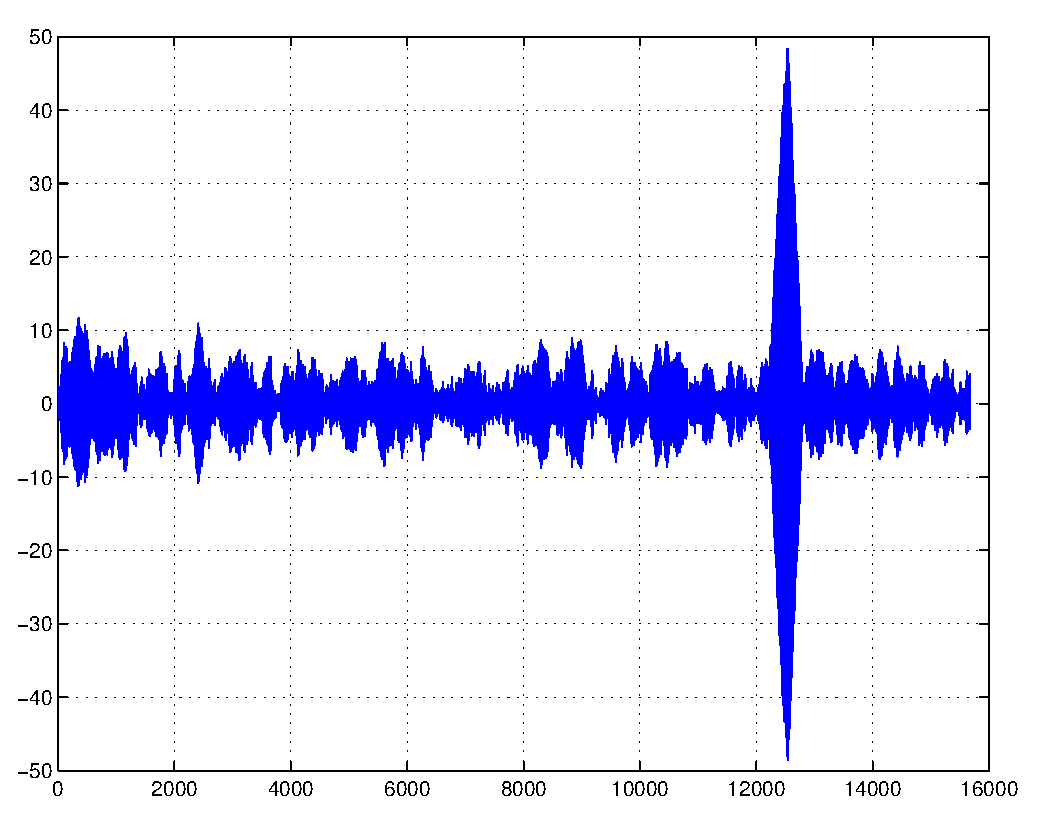
\includegraphics[width=\linewidth]{inc/8.eps}

		\item
			Autokorelační koeficienty jsem spočítal funkcí \texttt{xcorr} a~výsledek jsem
			vydělil počtem vzorků, aby to odpovídalo zadanému vztahu
			$ R[k] = \frac{1}{N} \sum\limits_n x[n] x[n+k] $.
			\\ 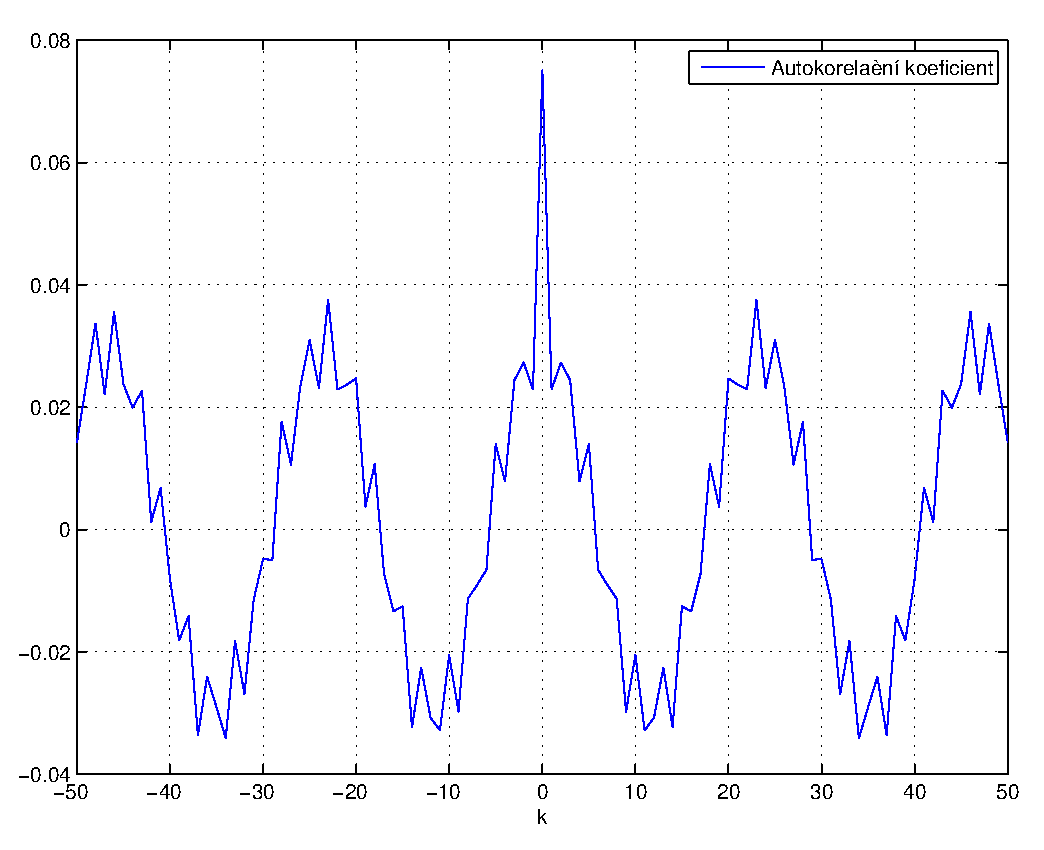
\includegraphics[width=\linewidth]{inc/9.eps}

		\item
			Hodnota koeficientu $ R[10] $ je $ \mathbf{-0.020553} $.

		\item
			Inspiroval jsem se algoritmem funkce \texttt{hist2} implementovaném v~souboru
			\texttt{hist2opt.m} ze studijní etapy k~projektu. Obrázek jsem vytvořil funkcí \texttt{imagesc}.
			\\ 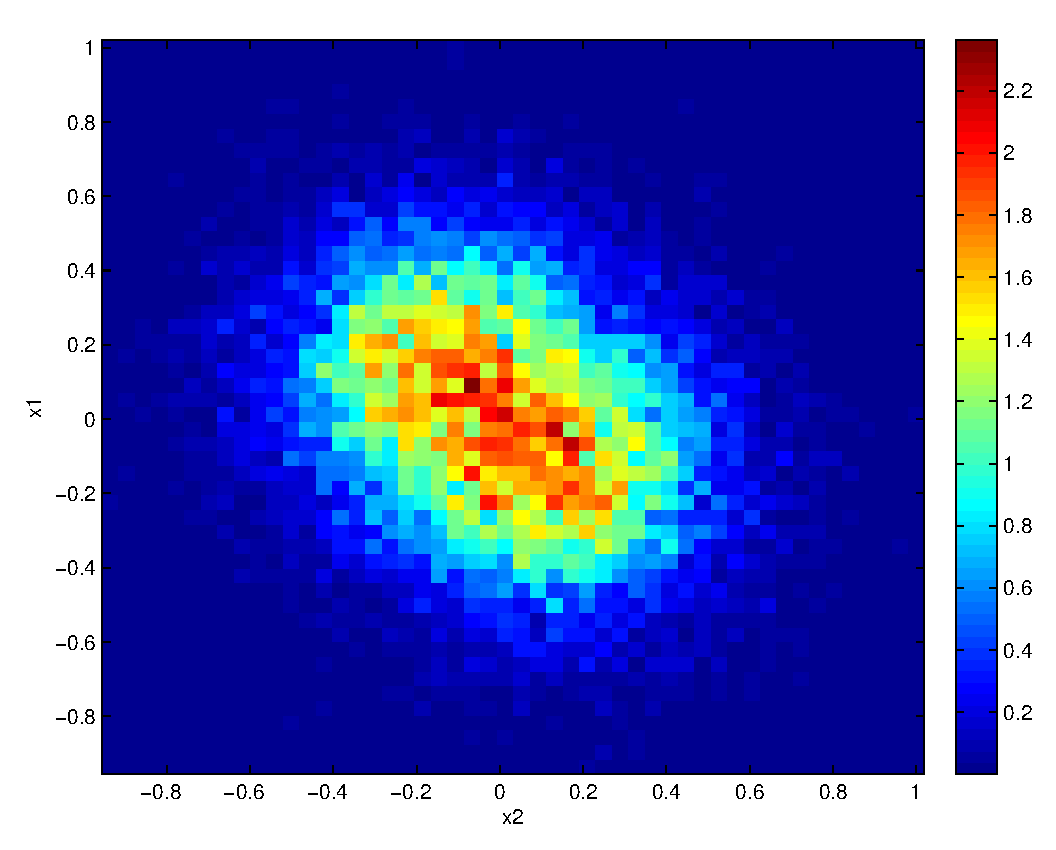
\includegraphics[width=\linewidth]{inc/11.eps}

		\item
			Ověření, zda se jedná o~správnou sdruženou funkci hustoty rozdělení pravděpodobnosti
			jsem provedl výpočtem $ \int_{x_1} \int_{x_2} p(x_1, x_2, 10) dx_1 dx_2 = 1 $.
			Výpočet jsem provedl tak, jak je to udělané ve funkci \texttt{hist2} implementované
			v~souboru \texttt{hist2opt.m} ze studijní etapy k~projektu. Získal jsem výsledek
			$ \mathbf{0.999375} $, z~čehož usuzuji, že se \textbf{jedná o~správnou sdruženou
			funkci hustoty rozdělení pravděpodobnosti}, pokud budu tolerovat určitou zaokrouhlovací chybu.

		\item
			Hodnota koeficientu $ R[10] $ je $ \mathbf{-0.020562} $. Výpočet jsem provedl tak,
			jak je to udělané ve funkci \texttt{hist2} implementované v~souboru \texttt{hist2opt.m}
			ze studijní etapy k~projektu. Pokud bych měl výsledek srovnat s~výsledkem z~úlohy~10,
			\textbf{řekl bych, že hodnoty jsou ekvivalentní}, pokud budu tolerovat určitou zaokrouhlovací
			chybu.
	\end{enumerate}


\end{document}
